\documentclass[tikz,border=3mm]{standalone}
\usepackage{pgfplots}
\usepgfplotslibrary{fillbetween}
\usetikzlibrary{patterns}
\pgfplotsset{compat=1.17}
\begin{document}
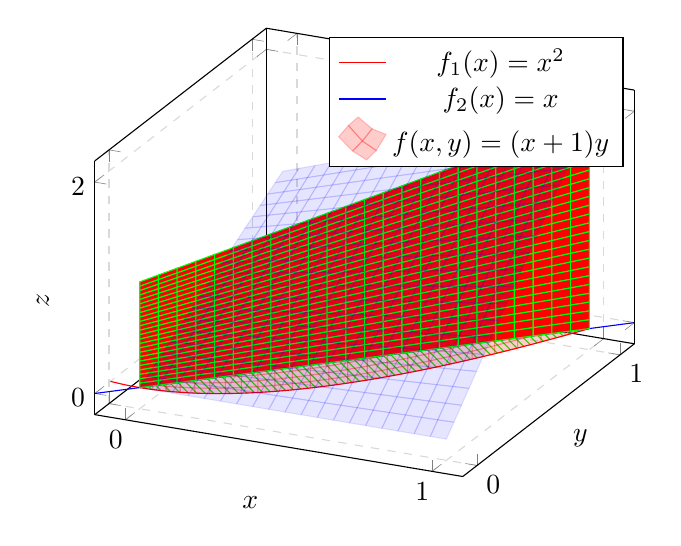
\begin{tikzpicture}
\begin{axis}[
    grid,
    grid style={dashed,gray!30},
    smooth,
    xmin=-0.1, xmax=1.1,
    ymin=-0.1, ymax=1.1,
    %axis lines=middle,
    xlabel=$x$,
    xlabel style={below, anchor=north east,inner xsep=0pt},
    xtick={-1,...,2},
    ylabel=$y$,
    ylabel style={above,anchor=south,inner ysep=0pt},
    ytick={-1,...,2},
    zlabel=$z$,
    ztick={0,2,10},
]


\addplot[red,name path=f1,mark=none,domain=-0.1:1,line legend] {x^2};
\addlegendentry{$f_{1}(x)=x^2$}

\addplot[blue,name path=f2,mark=none,domain=-0.1:1.1, line legend] {x};
\addlegendentry{$f_{2}(x)=x$}

\addplot3[surf,opacity=0.2,color=red,faceted color=red,domain=-0:1,y domain=0:1]({x},{x^2},{y*(x+1)});
\addplot3[surf,color=red,faceted color=green,opacity=1,domain=-0:1,y domain=0:1]({x},{x},{y*(x+1)});
\addplot3[surf,name path=z,faceted color=blue,color=blue,samples=20,domain=-0:1,opacity=0.1]{(x+1)*y};
\addlegendentry{$f(x,y)=(x+1)y$}




\path[name path=lower,intersection segments={of=f1 and f2,sequence=B0 -- A1}];
\addplot[pattern=north west lines, pattern color=green]fill between[of=f2 and lower];


\end{axis}
\end{tikzpicture}
\end{document}
